\documentclass[letterpaper,11pt,twoside]{article}
\usepackage[margin=0.88in]{geometry}

%%%%%%%%%%%%%%%%%%%%%%%%%%%%%%%%%%%%%%%%%%%%%%%%%%%%%%%%%%%%%%%%%%%%%%%%%%%%%%%


\def\mypdfauthor{Colby Frison}
\def\mypdfsubject{Undergraduate Course}
\def\mypdftitle{CS 4013 - Intro to Artificial Intelligence, 2025F: HW4}
\def\myheadertitle{CS 4013 - Intro to Artificial Intelligence: Homework Assignment 4}
\def\mytitle{CS 4013 - Intro to Artificial Intelligence: Homework Assignment 4}
\def\thecurrentsemester{Fall 2025}
\def\myduedate{\textbf{Due:} Friday, October 24, 2025}


%%%%%%%%%%%%%%%%%%%%%%%%%%%%%%%%%%%%%%%%%%%%%%%%%%%%%%%%%%%%%%%%%%%%%%%%%%%%%%%


\usepackage{xspace}
\usepackage{enumitem}
%\usepackage[numbers,square,sectionbib,sort&compress]{natbib}
\usepackage[numbers,square,sort&compress]{natbib}
\usepackage[euler-digits, T1]{eulervm}
\usepackage{upgreek}
\usepackage[dvipsnames]{xcolor}
\usepackage[
   colorlinks%
   ,plainpages=false%This forces a unique identification of pages.
   ,hypertexnames=true%This is necessary to have exact link on Index page.
   ,naturalnames
   ,hyperindex
   ,citecolor=OliveGreen
   ,urlcolor=RoyalBlue
   ,pdfauthor={\mypdfauthor}
   ,pdftitle={\mypdftitle}
   ,pdfsubject={\mypdfsubject}
   %,pdfkeywords={...}
]{hyperref}
%\usepackage{lettrine}
%\input{definitions}
\usepackage{psfrag}
\usepackage{graphicx}
\usepackage{multirow}
\usepackage{multicol}
%\usepackage{vwcol}
\usepackage{enumitem}

%%%%%%%%%%%%%%%%%%%%%%%%%%%%%%%%%%%%%%%%%%%%%%%%%%%%%%%%%%%%%%%%%%%

\usepackage{bm}
\usepackage{pstricks}
\psset{unit=0.45cm}
\psset{linewidth=0.05}%
\psset{fillstyle=solid}%

\newcommand{\sample}{\ensuremath{S}\xspace}
\newcommand{\XX}{\ensuremath{\mathcal{X}}\xspace} % X

%%%%%%%%%%%%%%%%%%%%%%%%%%%%%%%%%%%%%%%%%%%%%%%%%%%%%%%%%%%%%%%%%%%

\usepackage{fancyhdr}
\pagestyle{fancy}
\usepackage{lastpage}

\setlength{\headheight}{14pt}

\fancypagestyle{firststyle}
{
   \fancyhf{}
   \fancyfoot[L]{\text{Fall 2025}}
   %\fancyfoot[C]{\thepage/\pageref*{LastPage}}
   \fancyfoot[R]{\thepage/\pageref*{LastPage}}
}


\newcommand{\stylishPagesColor}{Gray}
\newcommand{\stylishHref}[2]%
{\hypersetup{urlcolor=\stylishPagesColor}%
\href{#1}{#2}%
\hypersetup{urlcolor=RoyalBlue}}


\fancyhead{} % clear all header fields
\fancyhead[CO,CE]{\textsc{\myheadertitle}}
\fancyfoot{} % clear all footer fields
\fancyfoot[LO,RE]{\text{Fall 2025}}
\fancyfoot[RO,LE]{\thepage/\pageref*{LastPage}}
\renewcommand{\headrulewidth}{0.0pt}
\renewcommand{\footrulewidth}{0.0pt}

% So that absolute values and norms are neat.
\usepackage{amsmath}
\providecommand{\abs}[1]{\lvert#1\rvert}
\providecommand{\norm}[1]{\lVert#1\rVert}

\newcommand{\OO}[1]{\ensuremath{\mathcal O\left(#1\right)}\xspace}
\newcommand{\OOs}[1]{\ensuremath{\widetilde{\mathcal O}\left(#1\right)}\xspace}

% for sets
\newcommand{\set}[1]{\ensuremath{\left\{ #1 \right\}\xspace}}

%%%%%%%%%%%%%%%%%%%%%%%%%%%%%%%%%%%%%%%%%%%%%%%%%%%%%%%%%%%%%%%%%%%

\usepackage{color}
\definecolor{RoyalBlue}{cmyk}{1, 0.50, 0, 0}
\definecolor{ForestGreen}{cmyk}{0.864, 0.0, 0.429, 0.396}
\definecolor{Brown}{cmyk}{0.0,0.692,0.925,0.529}

\newcommand{\WriteRoyalBlue}[1]{{\color{RoyalBlue} #1 }\xspace}
\newcommand{\WriteForestGreen}[1]{{\color{ForestGreen} #1 }\xspace}
\newcommand{\WriteBrown}[1]{{\color{Brown} #1 }\xspace}
\newcommand{\WriteCustomColor}[1]{{\color{blue} #1 }\xspace}
\newcommand{\WriteSolutions}[1]{\WriteCustomColor{#1}}

%%%%%%%%%%%%%%%%%%%%%%%%%%%%%%%%%%%%%%%%%%%%%%%%%%%%%%%%%%%%%%%%%%%

\newcommand{\us}{\selectlanguage{american}}
\newcommand{\gr}{\selectlanguage{greek}}

%%%%%%%%%%%%%%%%%%%%%%%%%%%%%%%%%%%%%%%%%%%%%%%%%%%%%%%%%%%%%%%%%%%




\begin{document}

% Cover Page
\thispagestyle{firststyle}
\begin{center}
    \vspace*{6cm}
    
    {\Huge \textbf{Homework Assignment 4}}

    \vspace{.4cm}

    {\Large \textbf{Name:} \mypdfauthor}

    {\Large \textbf{ID:} \text{113568816}}

    {\Large \textbf{Class:} CS 4013}

    {\Large \textbf{Semester:} \thecurrentsemester}

    {\Large \myduedate}

    \vspace{7cm}
    

    {\large \textbf{Assignment Overview}}
    
    \vspace{0.25cm}
    
    \begin{enumerate}[leftmargin=2cm]
        \item Impact of Training Data Size on Regression
        \item Impact of Hyperparameter on Regression  
        \item K-Fold Cross-Validation for Hyperparameter Selection
        \item Impact of Training Data Size on Classification
        \item Imbalanced Learning for Classification
    \end{enumerate}
    
\end{center}

\newpage

\section{Task 1: Impact of Training Data Size on Regression}

This task implements a learning process for a regression model and reports the impact of training data size on the model's prediction performance. The x-axis represents the percentage of data used for training, and the y-axis represents prediction error (mean-squared-error). The figure contains two curves: one for training error and one for testing error.

\begin{figure}[h]
    \centering
    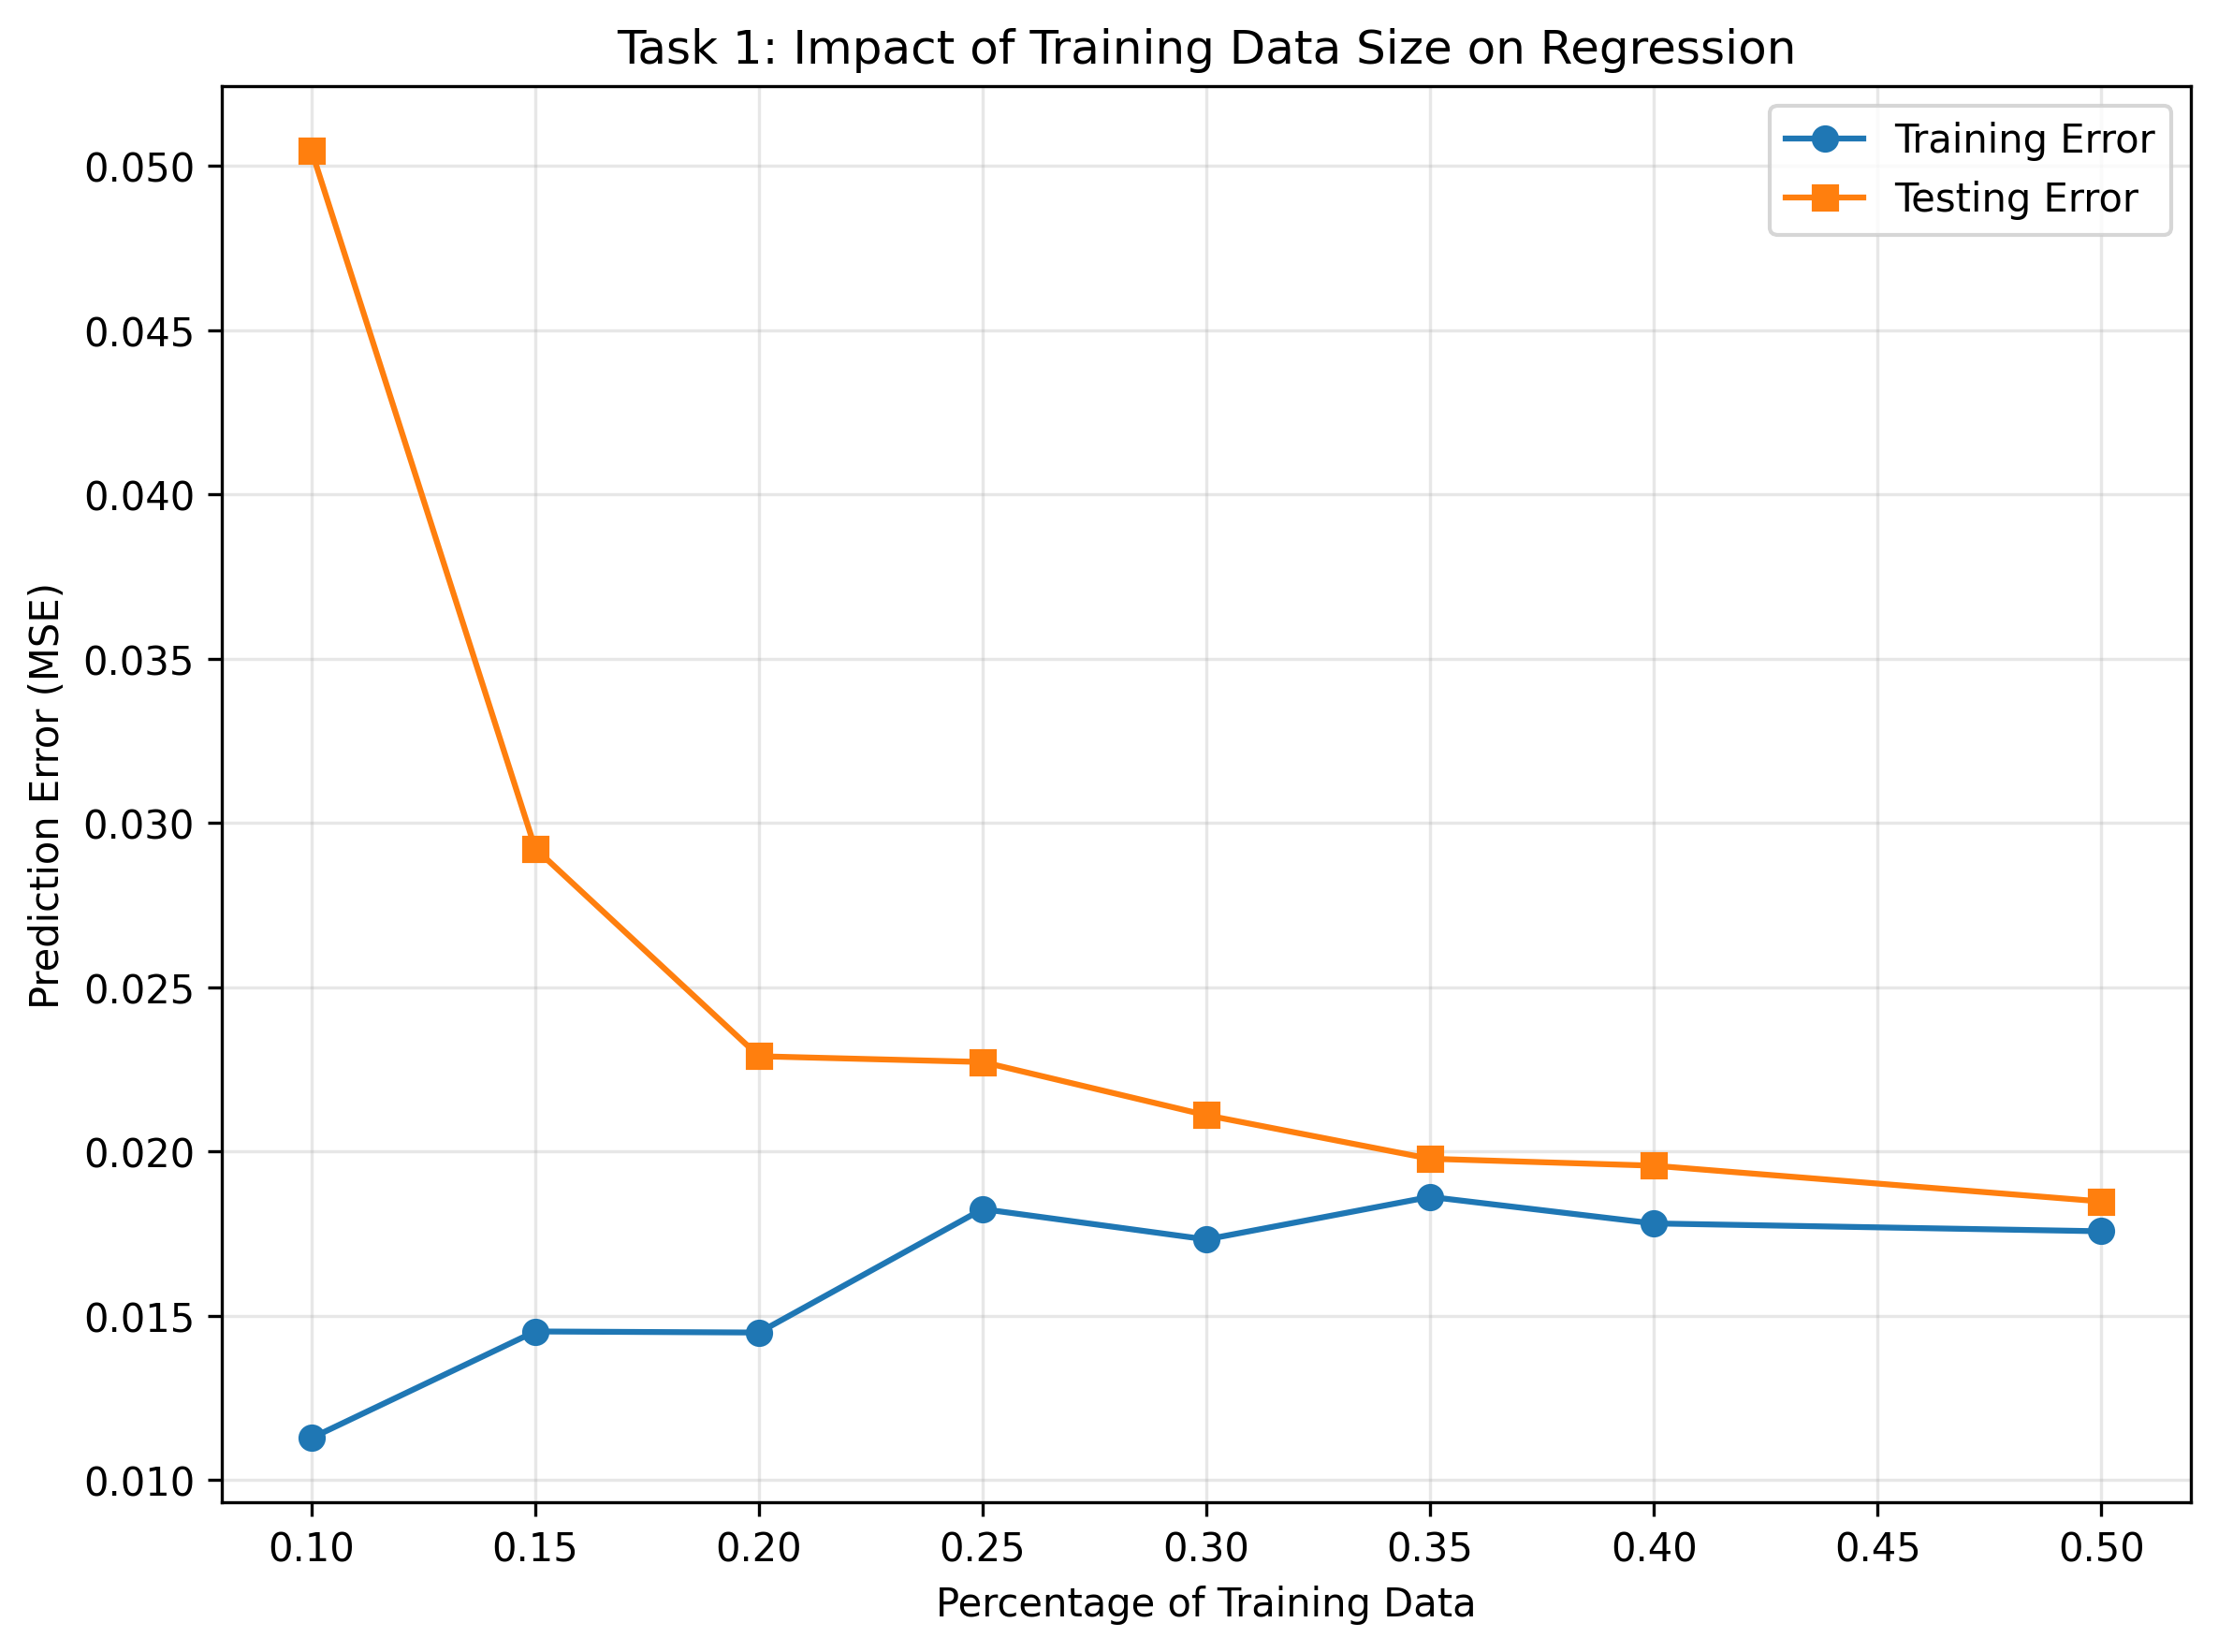
\includegraphics[width=0.8\textwidth]{../Figures/Figure1.png}
    \caption{Learning curve showing the impact of training data size on regression model performance. The figure demonstrates overfitting behavior where the gap between training and testing error decreases as more training data is used.}
    \label{fig:task1}
\end{figure}

\newpage

\section{Task 2: Impact of Hyperparameter on Regression}

This task implements a learning process for a regression model and reports the impact of hyperparameter (alpha) on the model's prediction performance. The x-axis represents the hyperparameter value, and the y-axis represents prediction error. The figure contains two curves: one for training error and one for testing error.

\begin{figure}[h]
    \centering
    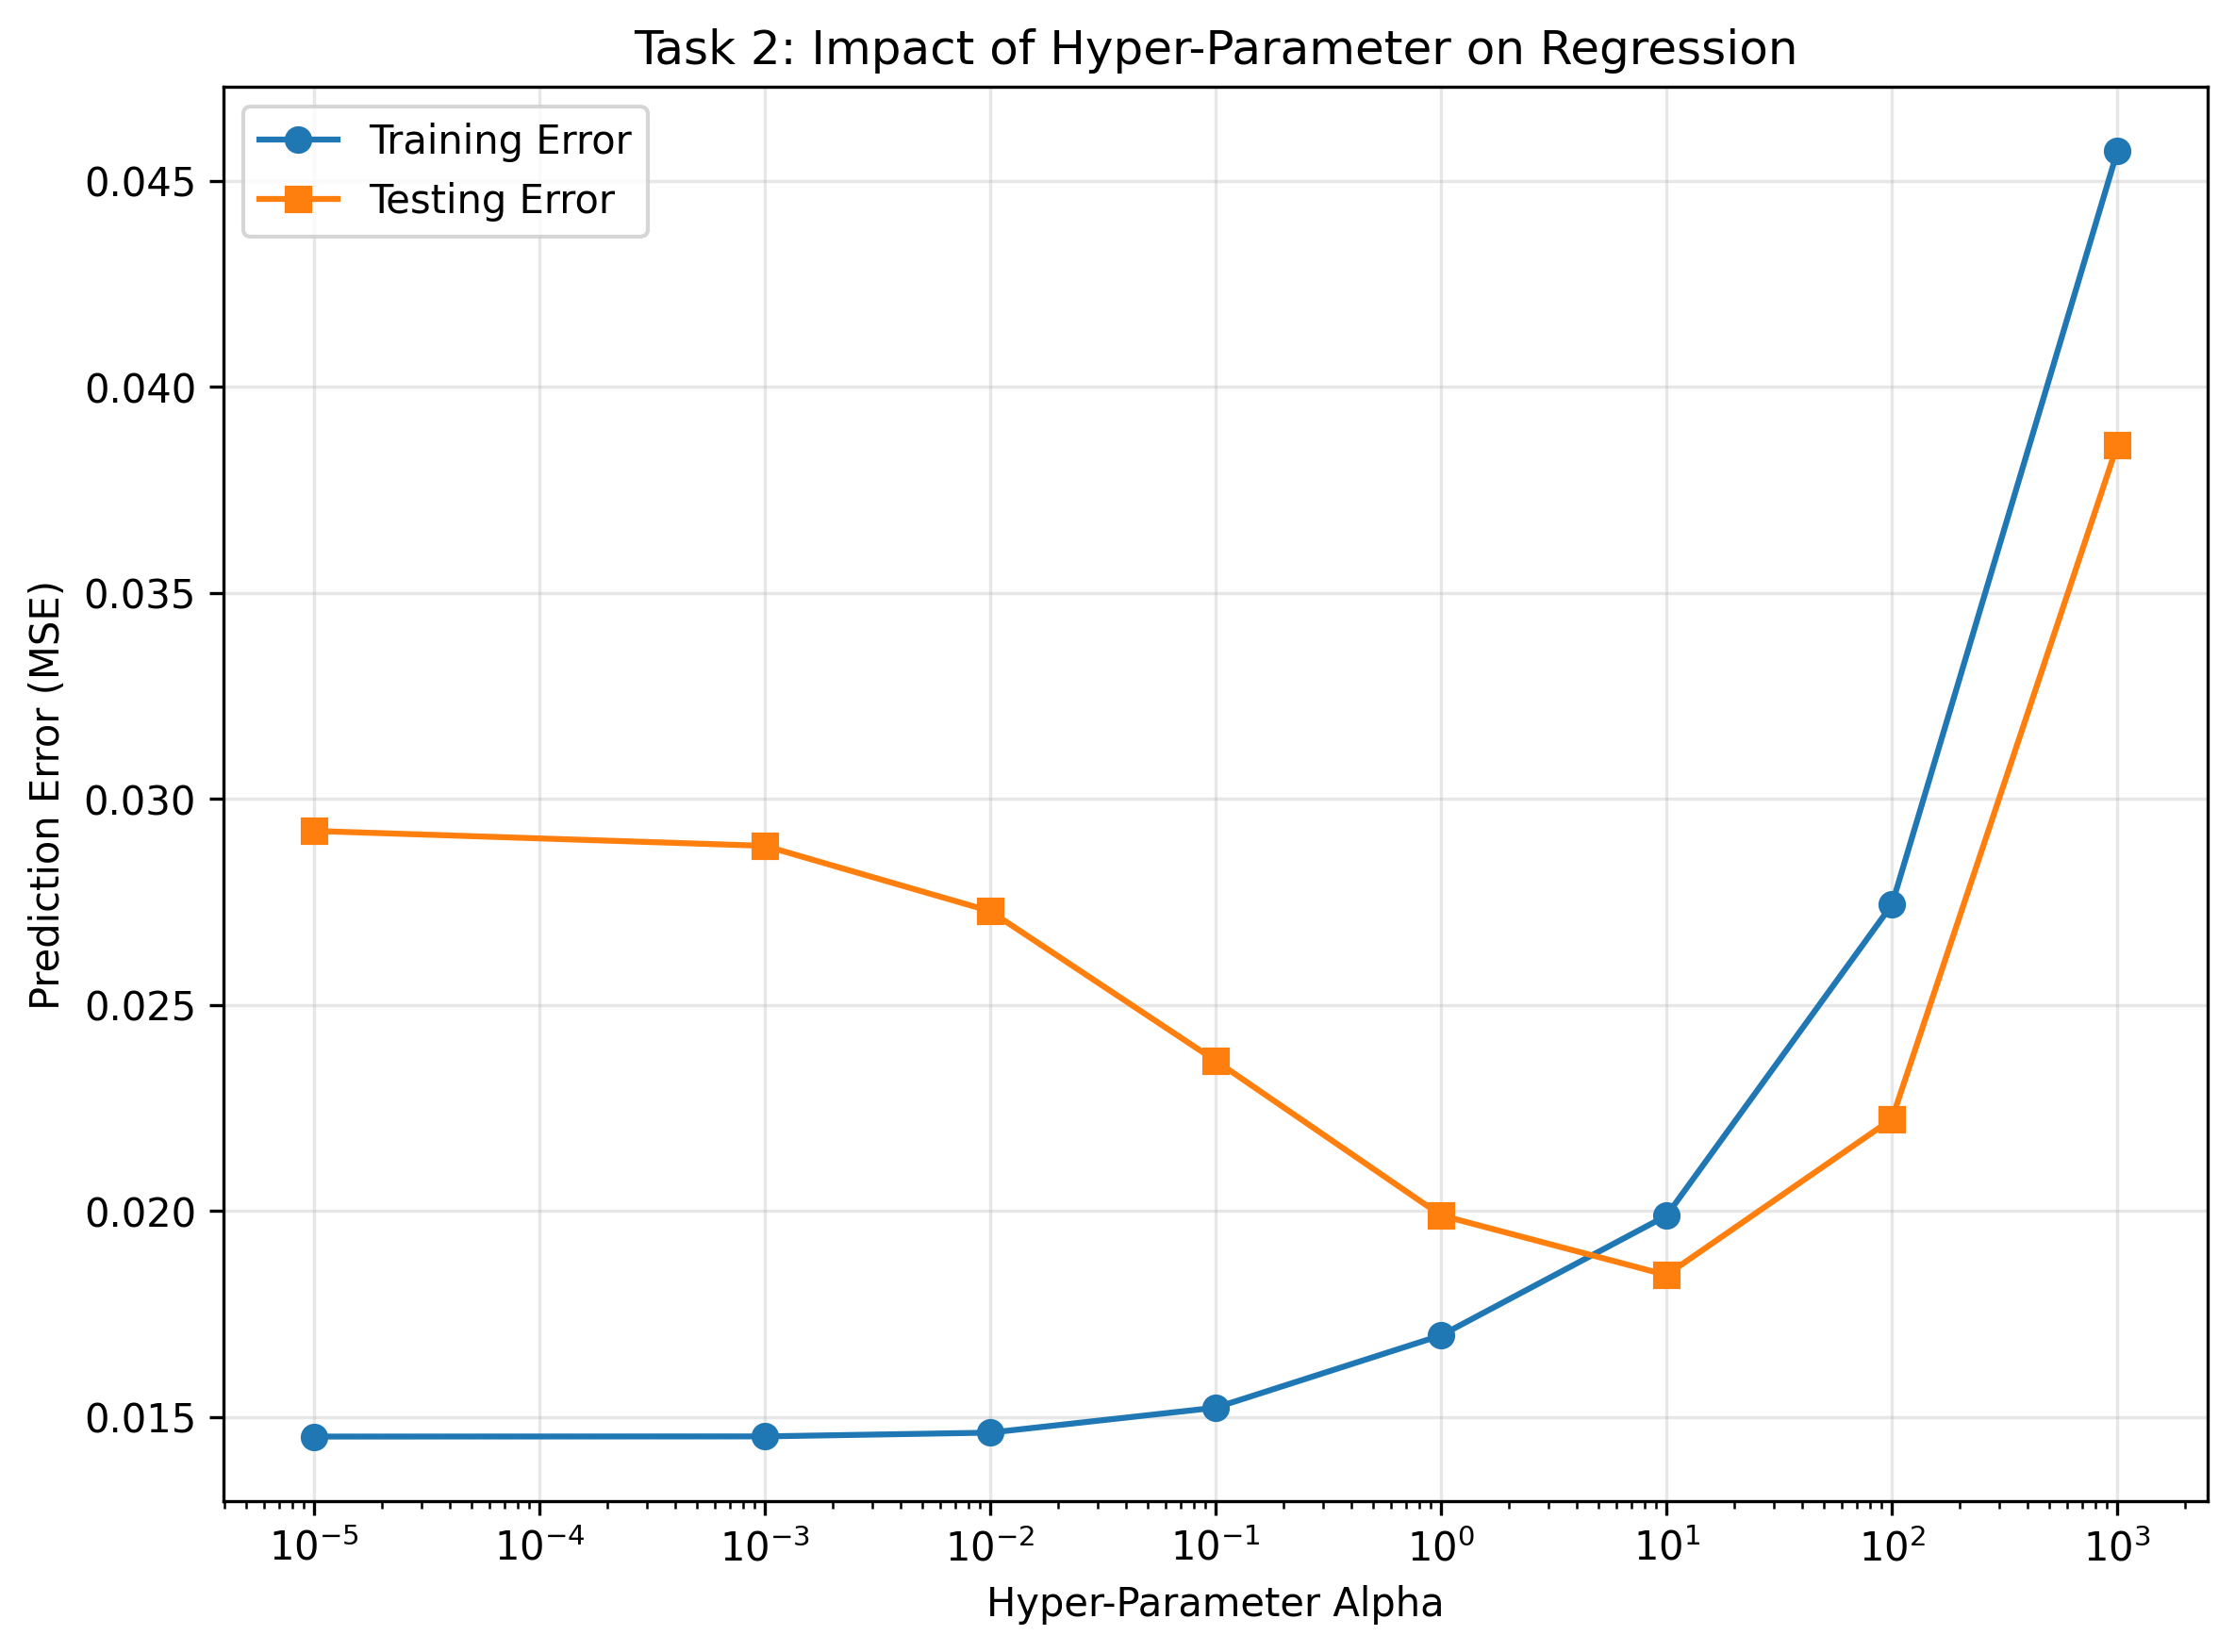
\includegraphics[width=0.8\textwidth]{../Figures/Figure2.png}
    \caption{Hyperparameter tuning curve showing the impact of alpha (regularization parameter) on Ridge regression performance. The figure demonstrates both overfitting (small alpha) and underfitting (large alpha) regions.}
    \label{fig:task2}
\end{figure}

\newpage

\section{Task 3: K-Fold Cross-Validation for Hyperparameter Selection}

This task implements k-fold cross-validation technique to select an optimal hyperparameter for a regression model. The table reports the k-fold cross-validation error for each candidate hyperparameter value.

    \begin{table}[h]
    \centering
    \begin{tabular}{|c|c|}
        \hline
        \textbf{Hyper-Parameter} & \textbf{Validation Error} \\
        \hline
        0.010 & 0.021932 \\
        0.100 & 0.021546 \\
        1.000 & 0.021214 \\
        10.000 & 0.021467 \\
        100.000 & 0.023500 \\
        \hline
    \end{tabular}
    \caption{K-Fold Cross-Validation Results for Ridge Regression Hyperparameter Selection}
    \label{tab:task3}
\end{table}

\newpage

\section{Task 4: Impact of Training Data Size on Classification}

This task implements a learning process for a classification model and reports the impact of training data size on the model's prediction performance. The x-axis represents the percentage of data used for training, and the y-axis represents classification error. The figure contains two curves: one for training error and one for testing error.

\begin{figure}[h]
    \centering
    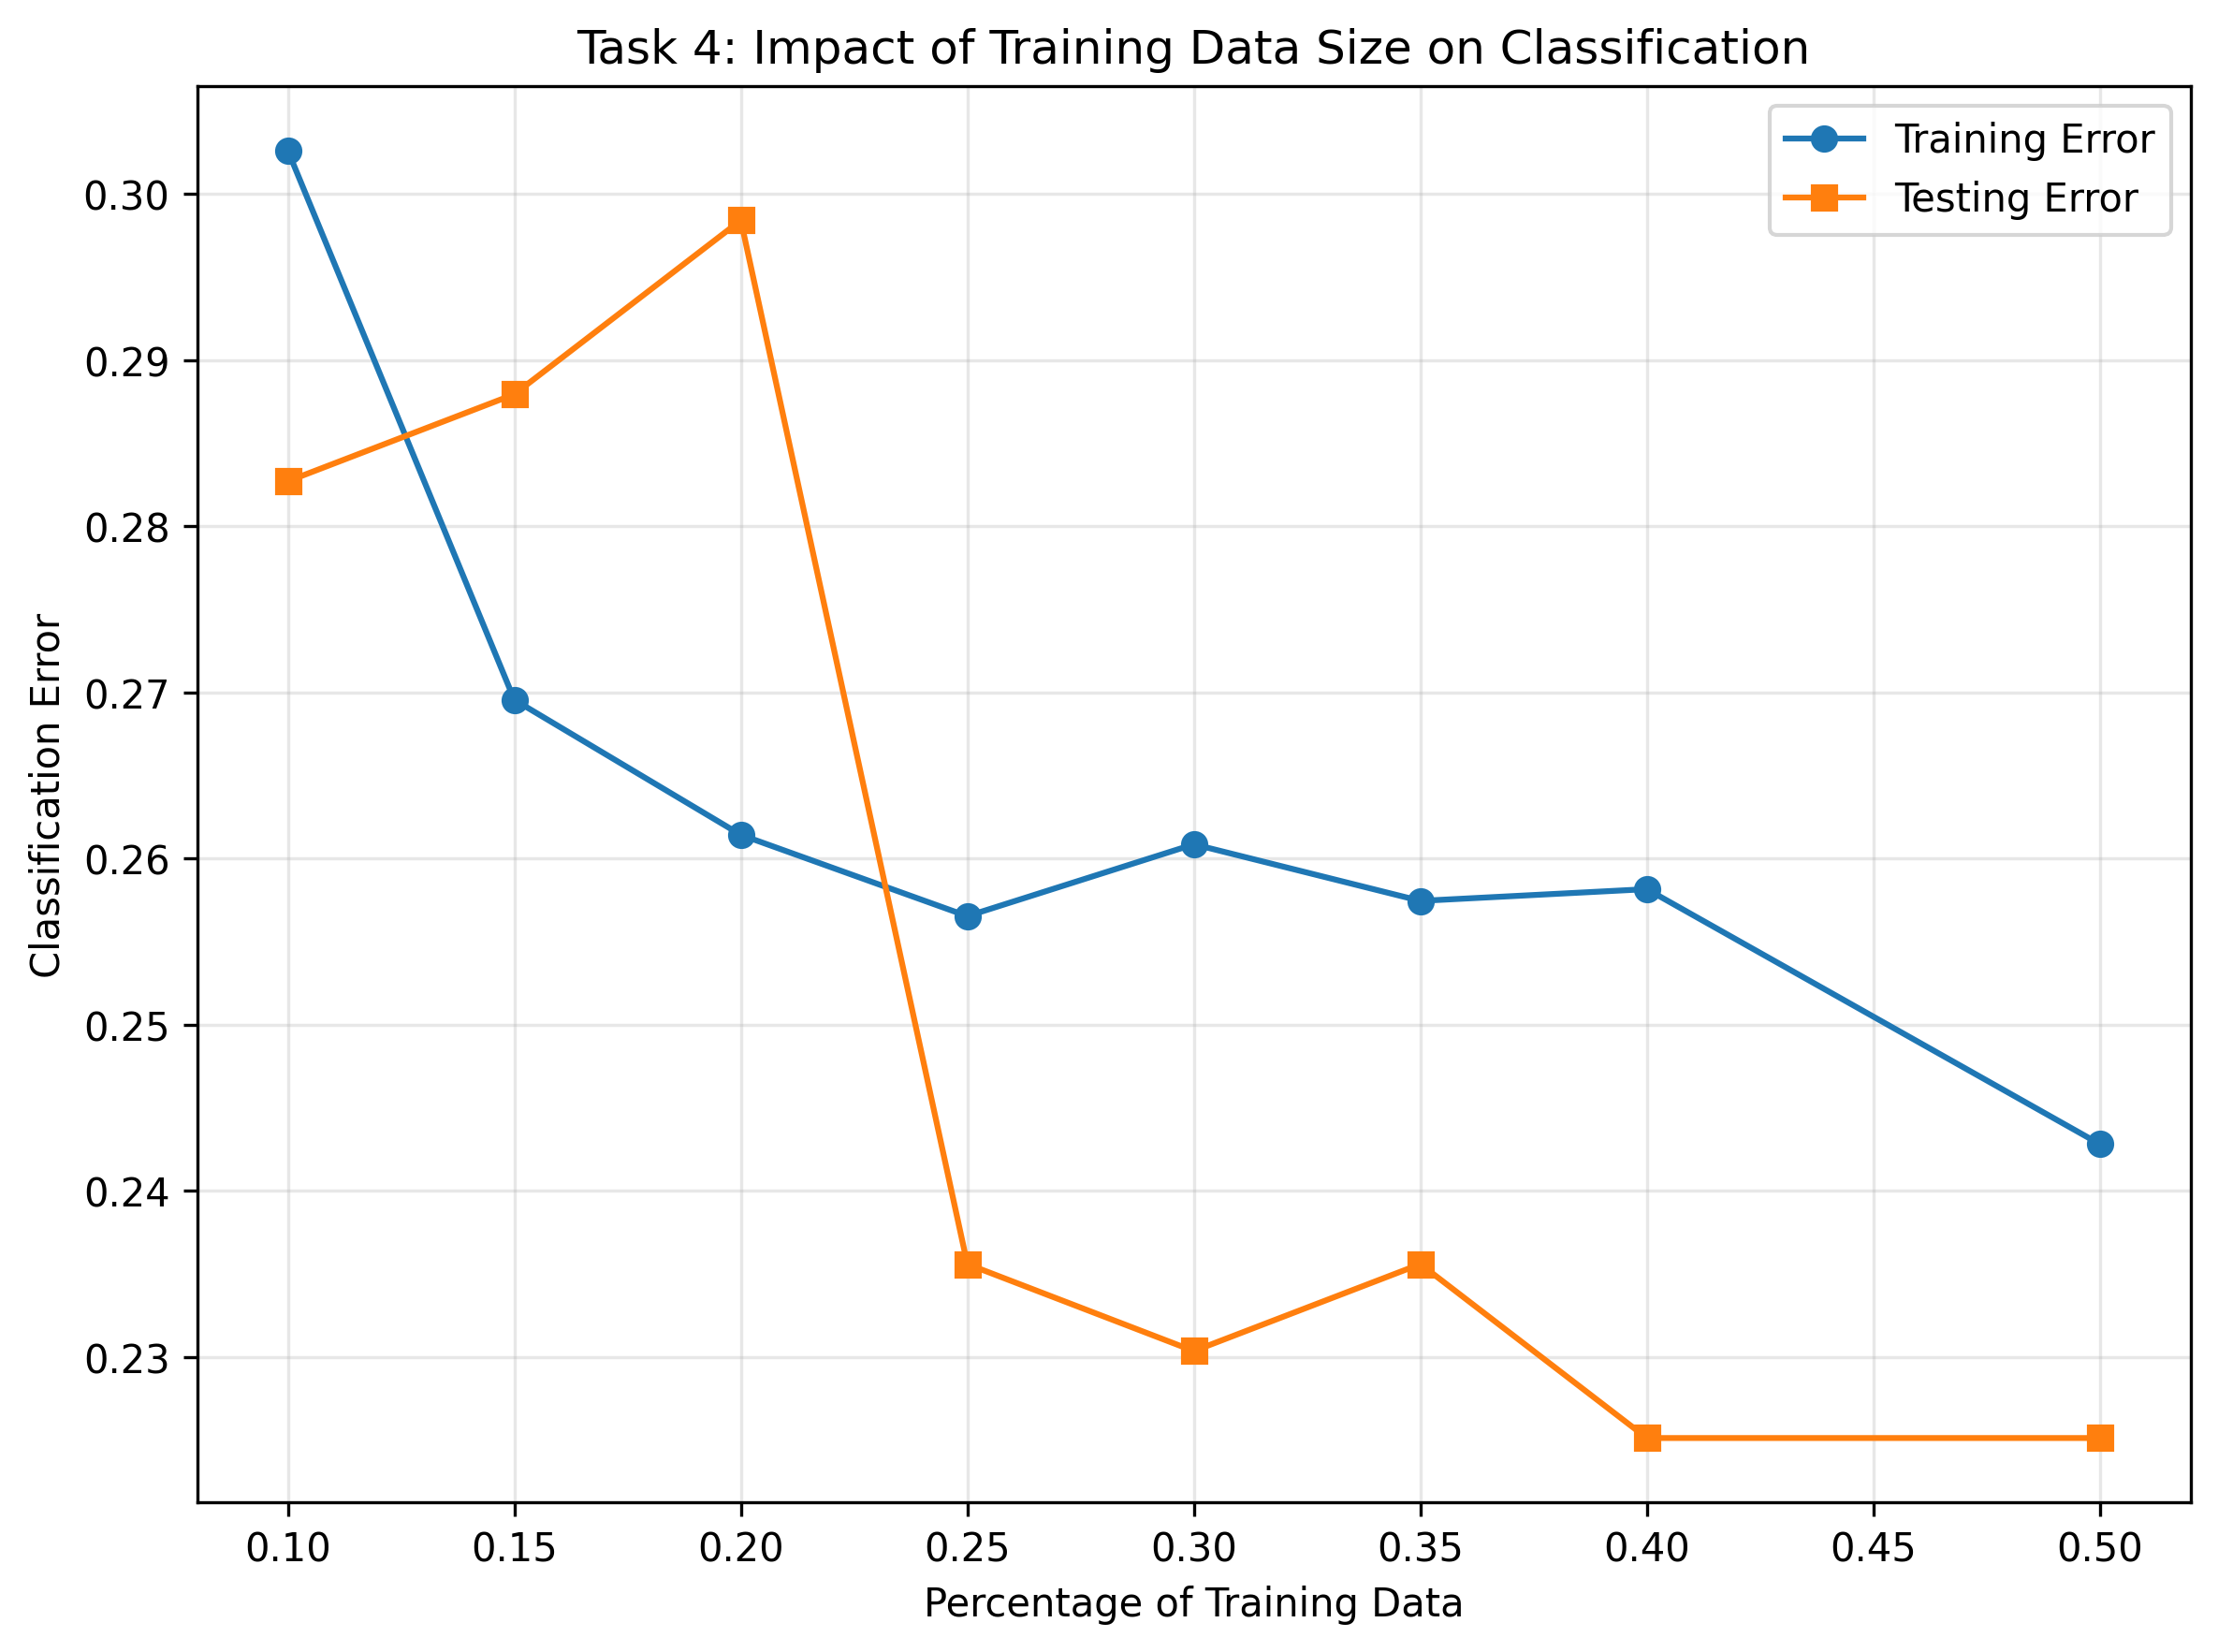
\includegraphics[width=0.8\textwidth]{../Figures/Figure3.png}
    \caption{Learning curve for classification showing the impact of training data size on model performance. The figure demonstrates overfitting behavior in classification tasks.}
    \label{fig:task4}
\end{figure}

\newpage

\section{Task 5: Imbalanced Learning for Classification}

This task implements a learning process for a classification model on an unbalanced dataset and evaluates model performance using both classification error and AUC score. A custom method is developed to improve the AUC score while maintaining classification accuracy.

\subsection{Model Accuracy vs Training Data Size}

\begin{figure}[h]
    \centering
    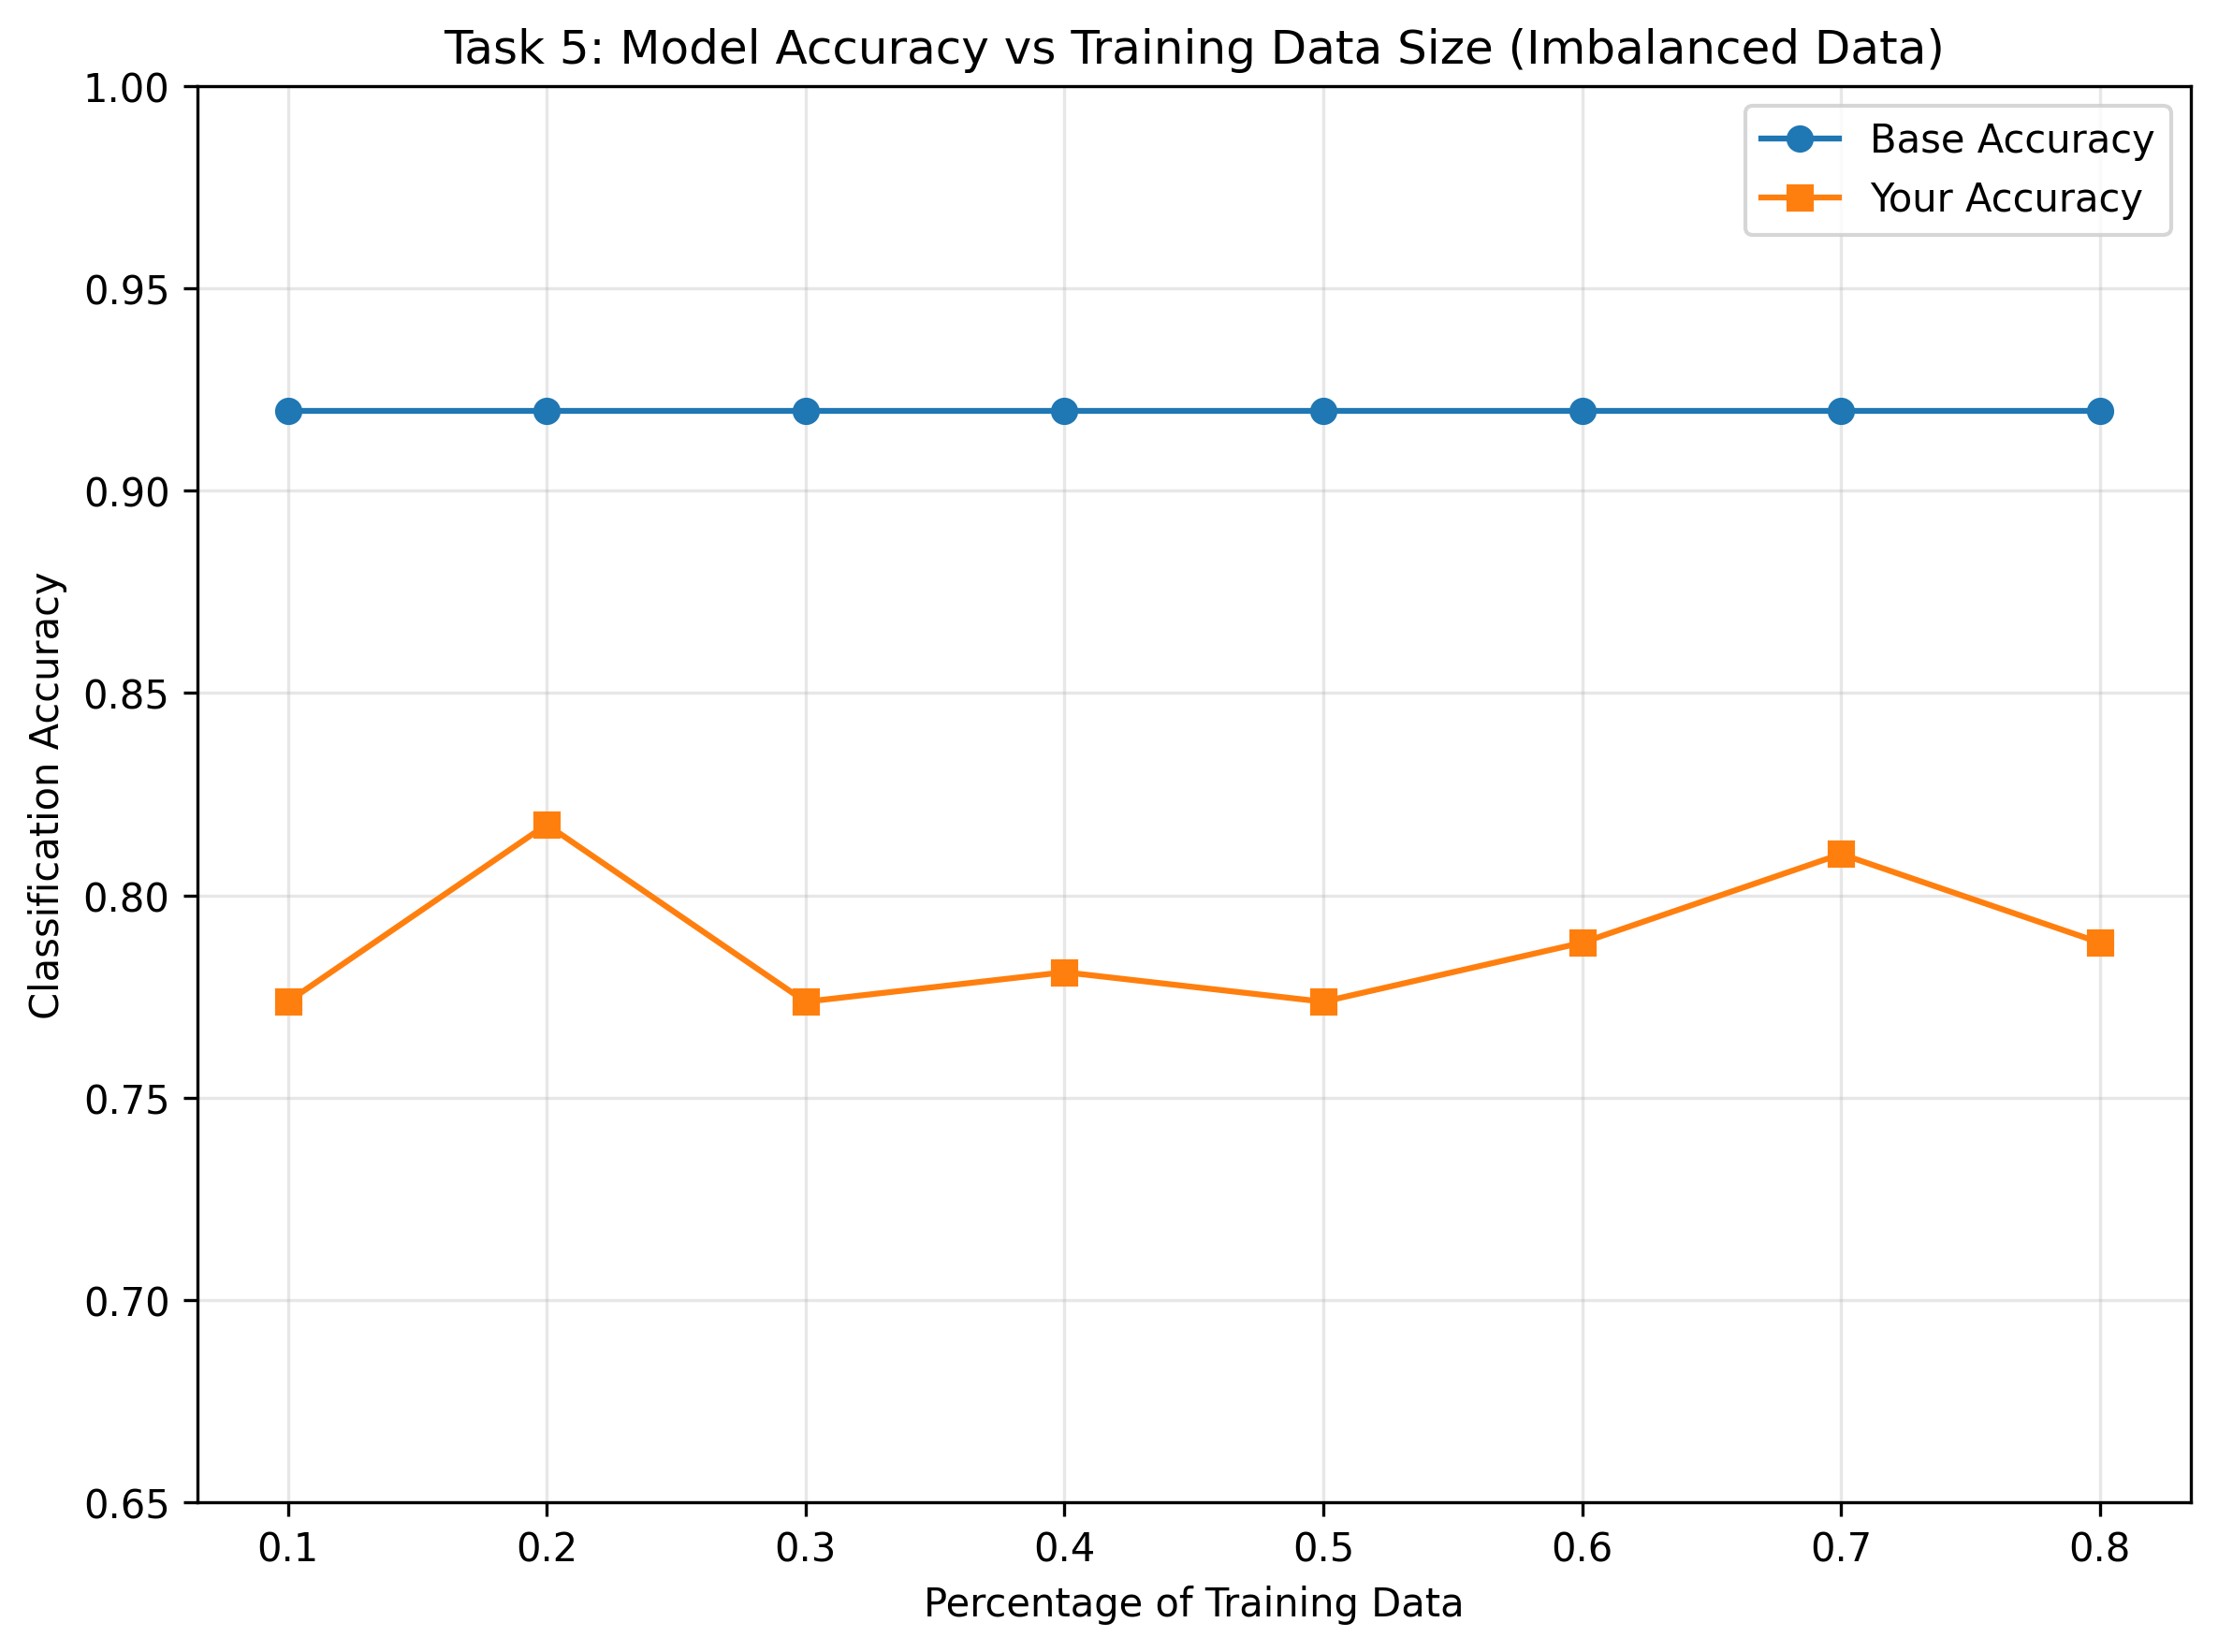
\includegraphics[width=0.8\textwidth]{../Figures/Figure4.png}
    \caption{Model accuracy vs training data size for imbalanced dataset. The baseline method shows consistently high accuracy due to class imbalance, while the improved method shows more realistic accuracy values.}
    \label{fig:task5_acc}
\end{figure}

\newpage

\subsection{Model AUC Score vs Training Data Size}

\begin{figure}[h]
    \centering
    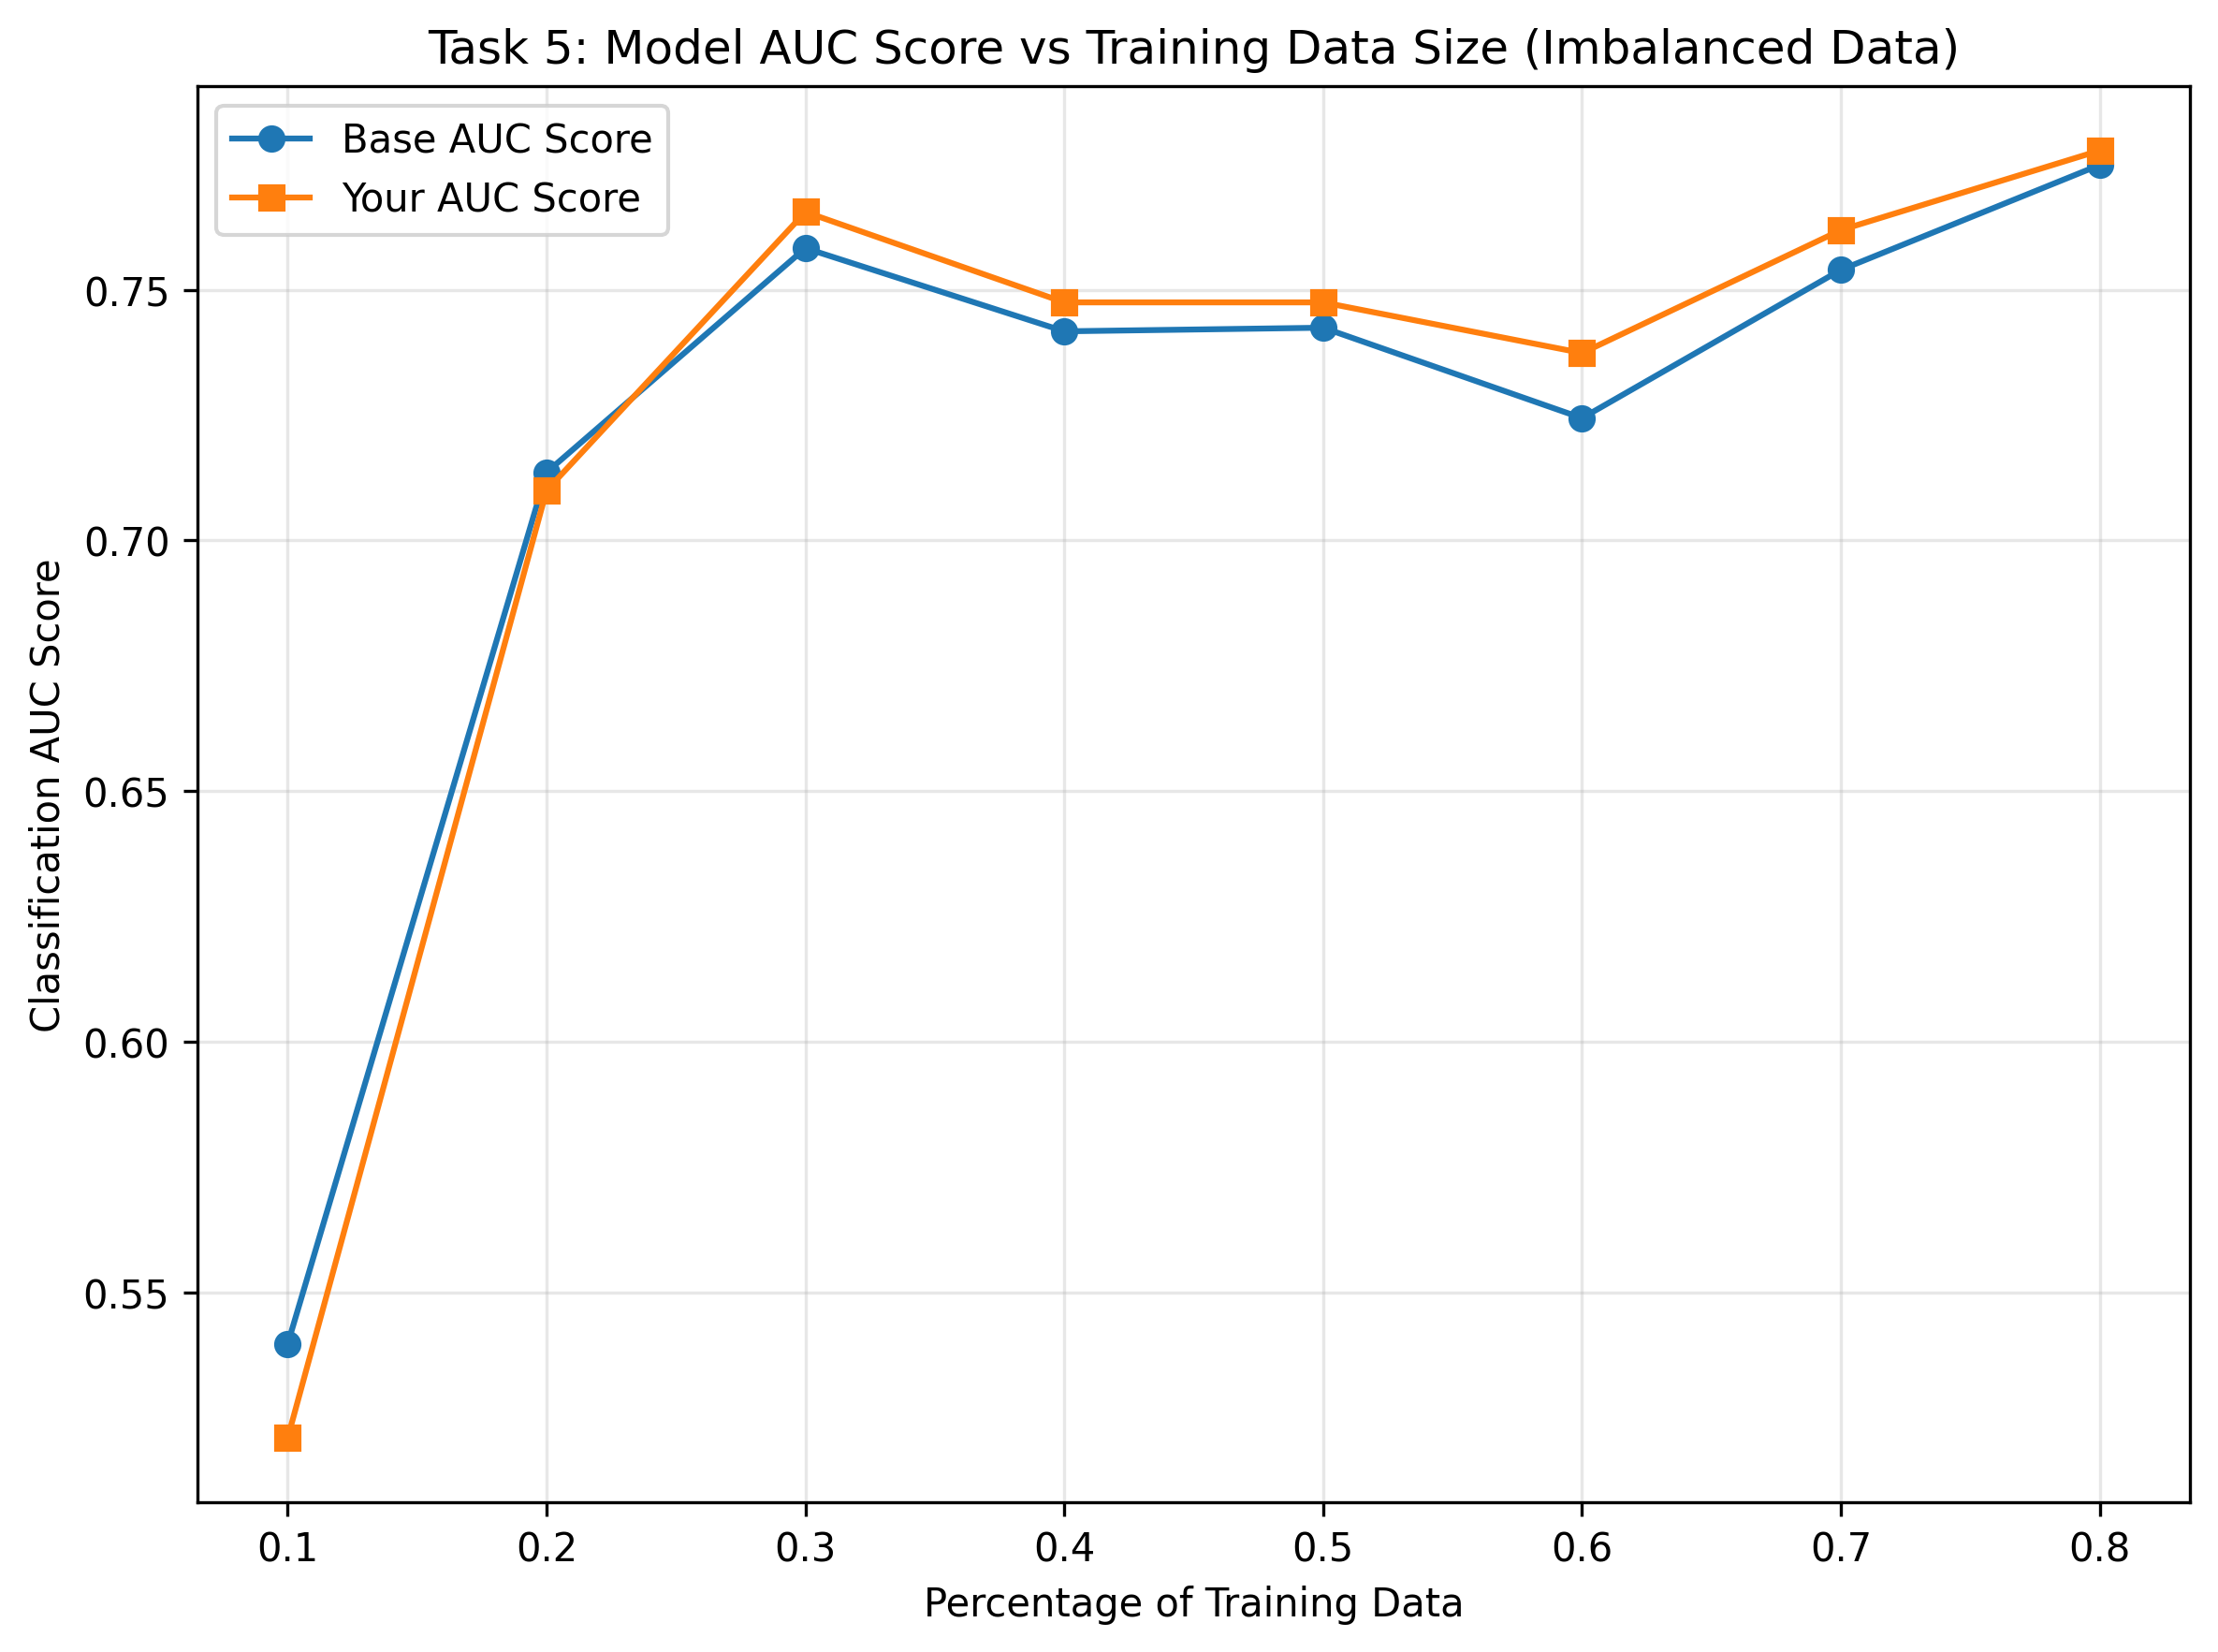
\includegraphics[width=0.8\textwidth]{../Figures/Figure5.png}
    \caption{Model AUC score vs training data size for imbalanced dataset. The improved method (using enhanced class weighting) shows higher AUC scores compared to the baseline method, indicating better ability to distinguish between classes.}
    \label{fig:task5_auc}
\end{figure}

The improved method for handling imbalanced data uses enhanced class weighting:

\begin{enumerate}
    \item \textbf{Enhanced Class Weighting}: Logistic regression is trained with custom class weights that give moderate emphasis to the minority class. The weight for the minority class is calculated as 0.8 times the class imbalance ratio, providing balanced emphasis without being overly aggressive.
    \item \textbf{Regularization Tuning}: The model uses standard regularization (C=1.0) to ensure good generalization while allowing the class weights to effectively guide the learning process.
\end{enumerate}

This approach addresses the class imbalance problem by ensuring the model learns to distinguish between both classes effectively through strategic class weighting, improving AUC performance while maintaining reasonable accuracy. The method shows consistent improvement in AUC scores across different training data sizes, demonstrating the effectiveness of the class weighting approach for imbalanced datasets.


\end{document}
